\section{BSSRDF parametrization}

Artists prefer to define surface albedo and mean multiple scattering distance
(characteristic or visible depth of the SSS). The radiative transport scattering
coefficients must therefore be inferred by inverting the diffusion equation.

\emph{mean-free path gives the scale of the response for a given material. For
two materials that differ only by $l$, we can predict the response of the second
material by scaling the response of the first material by the ratio of their
mean-free-paths.}


The scattering was parameterized by the volume scattering and absorption
coefficients $\sigma_s$ and $\sigma_a$ (or, equivalently, the volume
scattering albedo $\alpha = \sigma_s/\sigma_t = \sigma_s/(\sigma_s + \sigma_a)$
and volume mean free path length $l = 1/\sigma_t = 1/(\sigma_s + \sigma_a)$.)
In follow-up work, Jensen and Buhler \cite{Jensen:2002:RHR:566570.566619}
introduced a more intuitive parameterization of subsurface scattering:
surface albedo (diffuse surface reflectance) $A = \int\limits_0^\infty
R(r)2\pi r dr$ and diffuse mean free path length $l_d$ on the surface.

In contrast, BSSRDF profile for the diffusion approximation proposed by Burley
and Christensen relays on \textit{surface albedo} (diffuse surface reflectance)
$A=\int_0^{\infty} R(r)2\pi rdr$ of the material.

There are ways of analytically computing \textit{surface albedo A} at a runtime
out of $\sigma_s$ and $\sigma_a$.

Overview of Jensan's approach. Compare with the following.

By rendering different materials with various oprical properties and using curve
fitting, I've come up to the following expression:
\[
A(\alpha) = a + b(1- e^{-c\alpha})
\]

with parameters $a = 0.0699, b = -3.97\cdot 10^{-05}, c =-10.0$

\begin{figure}
    \centering
    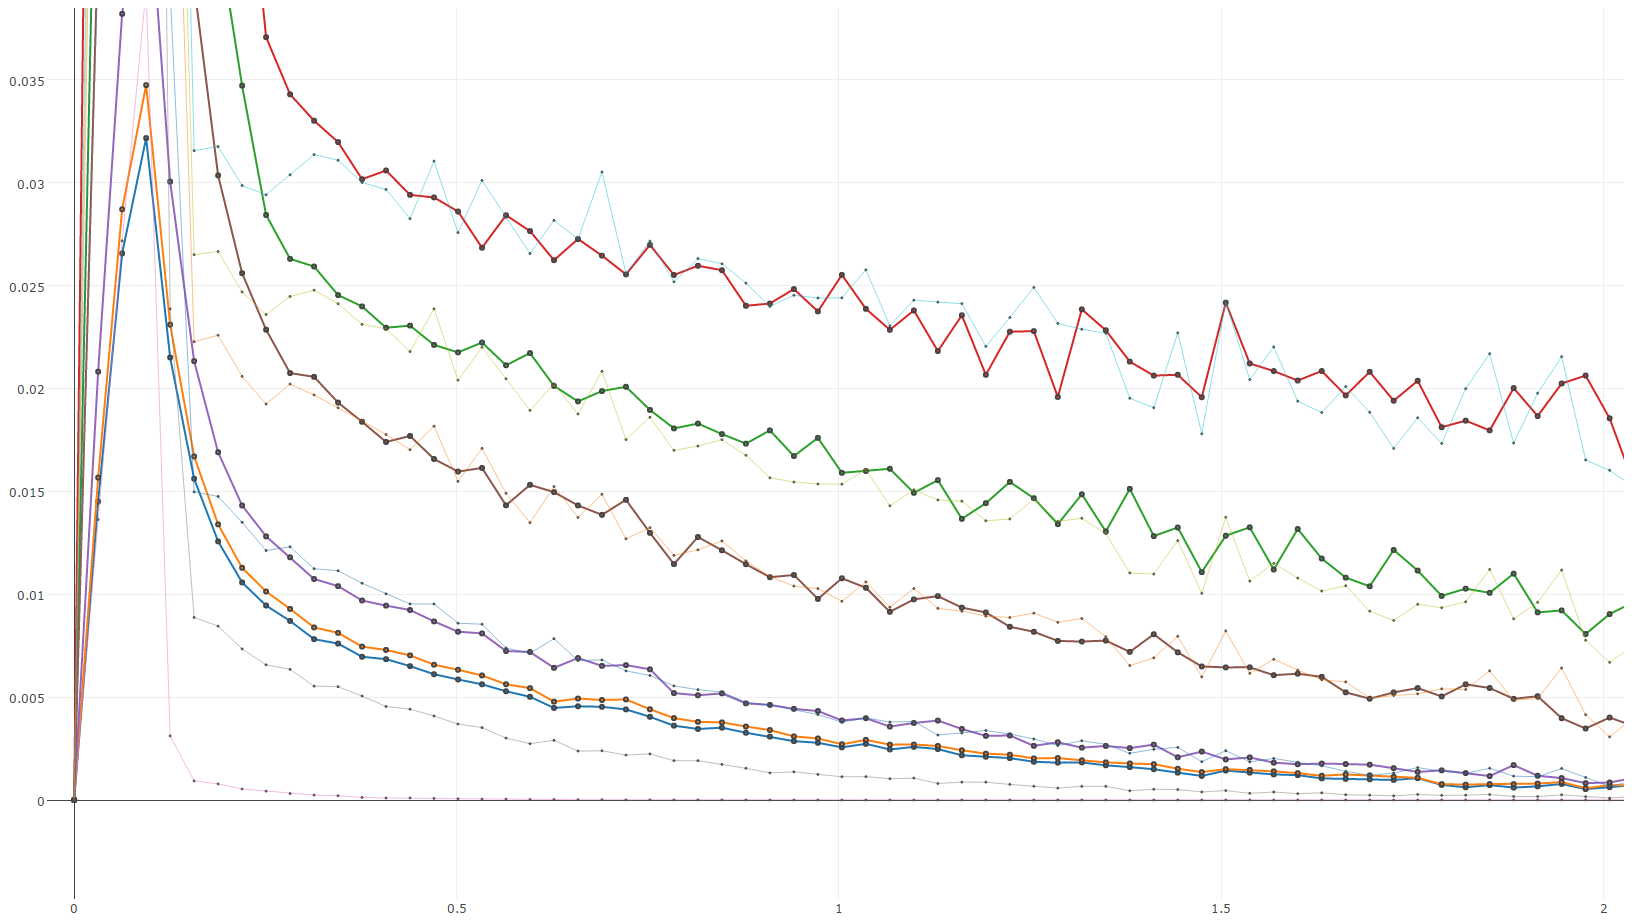
\includegraphics[width=0.9\textwidth]{imgs/plots/aA_fitting}
    \caption{The curve fitting results of the sigmas to albedo}
    \label{fig:albedo_fitting}
\end{figure}

The results from the following plot \ref{fig:albedo_fitting} show good match for
Burley profiles (thick lines) to Monte Carlo references (thin lines) for high albedo materials (top
four curves). But there is a significant difference for low albedo materials
with approximately $A<0.3$

Note that two lower thick lines does not not correspond to lower two thin lines.
And this result is consistent with the assumptions of the diffusion theory of
the light transport in participating media.